\documentclass[10pt]{article}



%%%%%%%%%%%%%%%%%%%%%%%%%%%%%%%%%%%%%%%%%%%%%%%%%%%%%%%%%%%%%%%%%%%%%%%%%%%%%%%%%%%%%%%%%%%%%%%%%%%%%%
%%%%%%%%%%%%%%%%%%%%%%%%%%%%%%%%%%%%%%%%BYTECODE LANGUAGE%%%%%%%%%%%%%%%%%%%%%%%%%%%%%%%%%%%%%%%%%%%%%%%%%%%
%%%%%%%%%%%%%%%%%%%%%%%%%%%%%%%%%%%%%%%%%%%%%%%%%%%%%%%%%%%%%%%%%%%%%%%%%%%%%%%%%%%%%%%%%%%%%%%%%%%%%%%%%%%%
 \newcommand{\bcIns}{\mbox{ \rm I} }
 \newcommand{\instrs}{\mbox{ \rm IS} }
 \newcommand{\ifCond}{ \instr{if\_cond } }
 \newcommand{\goto}{ \instr{goto } }
 \newcommand{\return}{ \instr{return } }
 \newcommand{\arithOp}{ \instr{arith\_op} }
 \newcommand{\load}{ \instr{load} }
 \newcommand{\store}{ \instr{store} }
 \newcommand{\push}{ \instr{push} }
 \newcommand{\pop}{\instr{pop}}
 \newcommand{\dup}{\instr{dup}}
 \newcommand{\iinc}{\instr{iinc}}
 \newcommand{\new}{\instr{new}}
 \newcommand{\newarray}{\instr{newarray}}
 \newcommand{\putfield}{\instr{putfield}} 
 \newcommand{\getfield}{\instr{getfield}}
 \newcommand{\arrstore}{\instr{type\_astore}} 
 \newcommand{\arrload}{\instr{type\_aload}}
 \newcommand{\arraylength}{\instr{arraylength}}
 \newcommand{\instanceof}{\instr{instanceof}} 
 \newcommand{\checkcast}{\instr{checkcast}} 
 \newcommand{\athrow}{\instr{athrow}}
 \newcommand{\invoke}{\instr{invoke}}
 \newcommand{\jsr}{\instr{jsr}}
 \newcommand{\ret}{\instr{ret}}
%%%%%%%%%%%%%%%%%%%%%%%%%%%%%%%%%%%%%%%%%%%%%%%%%%%%%%%%%%%%%%%%%%%%%%%%%%%%%%%%%%%%%%%%%%%%%%%%%%%%%%
%%%%%%%%%%%%%%%%%%%%%%%%%%%%%%%%%%%%%%%%BYTECODE LANGUAGE%%%%%%%%%%%%%%%%%%%%%%%%%%%%%%%%%%%%%%%%%%%%%%%%%%%
%%%%%%%%%%%%%%%%%%%%%%%%%%%%%%%%%%%%%%%%%%%%%%%%%%%%%%%%%%%%%%%%%%%%%%%%%%%%%%%%%%%%%%%%%%%%%%%%%%%%%%%%%%%%



\newcommand{\todo}[1]{\marginpar{\baselineskip0ex\rule{2,5cm}{0.5pt}\\[0ex]{\textsf{#1}}}}
\newcommand{\fig}[1]{ Fig.#1}
\newcommand{\jmlKey}[1]{\mbox{\rm\textbf{#1}}}% wrapping jml keywords
\newcommand{\java}[1]{\texttt{#1}}
\newcommand{\stack}[1]{\mbox{\rm\textbf{st}}(#1)}% element on top stack 
\newcommand{\stackOnly}{\mbox{\rm St}}
\newcommand{\stackOnlyParam}[1]{\mbox{\rm St}(#1)}
\newcommand{\newStack}{ \lbrack~\rbrack  } % empty stack
\newcommand{\update}[3]{ #1 [ \oplus {#2} \rightarrow {#3} ] }

\newcommand{\counter}{\mbox{\rm\textbf{cntr}} }
\newcommand{\counterOnly}{\mbox{\rm Cntr} }
\newcommand{\topStack}{\mbox{\rm cntr} }
\newcommand{\true}{\mbox{\rm\textbf{true}} } % true from the assertion language
\newcommand{\false}{\mbox{\rm\textbf{false}}} % false from the assertion language



\newcommand{\instr}[1]{\mbox{  \rm #1} }

%\newcommand{\loopStart}[1]{\textbf{loop\_start$\tt{_#1}$}}
%\newcommand{\loopEnd}[1]{\textbf{loop\_end$\tt{_#1}$}}
%\newcommand{\invariant}[1]{\it{I}_{\tt{#1}}}
%\newcommand{\boucle}[1]{\texttt{#1}}
%\newcommand{\loopModifies}[1]{\textbf{Modifies}(\texttt{#1}) }

\newcommand{\ins}[1]{instr_{#1}}
\newcommand{\insOnly}{\texttt{instr}}

% the grammar for the bytecode specification language
%\newcommand{\ClassSpec}{\rm{ClassSpec}}
%\newcommand{\ClassInv}{ClassInv}
%\newcommand{\ClassHistoryConstr}{ClassHistoryConstr}

%\newcommand{\MethodSpec}{\rm{MethodSpec}}


%\newcommand{\specCase}{\textrm{SpecCase}}
%\newcommand{\requires}{requires}
%\newcommand{\ensures}{ensures}
%\newcommand{\exsures}{exsures}
%\newcommand{\modifies}{modifies}

%\newcommand{\jmlStmt}[1]{\textrm{#1}}
%\newcommand{\specExpression}{\mathcal{E}^{spec}}

%\newcommand{\interMethodSpec}{\rm{InterMethodSpec}}
%\newcommand{\loopSpec}{\rm{loopSpec}}
%\newcommand{\assert}{\rm{assert}}

%\newcommand{\ArithExpr}{\texttt{ArithmeticExp} }

%\newcommand{\JMLExpr }{\texttt{JmlExp} }


\newcommand{\integer}{\texttt{int} }
\newcommand{\register}[1]{\mbox{\rm\textbf{reg}}(#1)}

\newcommand{\Mynull}{\jmlKey{null}}
\newcommand{\this}{\texttt{this}}
\newcommand{\fieldAccess}[2]{#1\mbox{\rm\textbf{.}}#2}
\newcommand{\arrayAccess}[2]{\mbox{\rm\textbf{arrayAccess}}( #1, #2) }  %{\mbox{\rm arrAccess}(#1, #2)}
\newcommand{\arrayAccessOnly}{\mbox{\rm arrAccess}}


%\newcommand{\loopInv}{loopInvariant}
%\newcommand{\loopMod}{loopModifies}

\newcommand{\result}{\jmlKey{$\backslash$result}}
%\newcommand{\old}[1]{\jmlKey{$\backslash$old(}#1\jmlKey{)}}
%\newcommand{\typeof}[1]{\jmlKey{$\backslash$typeof(}#1 \jmlKey{)}}
%\newcommand{\TYPE}{\jmlKey{TYPE} }
%\newcommand{\elemtype}[1]{ \jmlKey{$\backslash$elemtype(}#1\jmlKey{)} } 
%\newcommand{\excPost}{\psi^{exc}}

\newcommand{\Myspace}{\phantom{aaa}}
\newcommand{\predicate}{ \mathcal{P}} 
\newcommand{\Myfalse}{ \textit{false} }
\newcommand{\Mytrue}{ \textit{true} }



% abstractCtrlFlow.tex
\newcommand{\execRel}{\rightarrow} % the execution relation
\newcommand{\blockm}[1]{ \tt{b^{#1}} }
\newcommand{\blockSeq}[1]{ \tt{b_{seq}^{#1}} }
\newcommand{\pathm}[2]{\blockm{#1} \execRel^{*} \blockm{#2} }
\newcommand{\instrPost}[1]{ post(\instr{#1} )}
\newcommand{\invariant}{\textit{I}}




%from wp.tex
%\newcommand{\wpExeWithLoops}[1]{ \rm{Wp''}\rm{(#1)} }
%\newcommand{\wpExe}[1]{ \rm{Wp'}\rm{(#1)} }




\newcommand{\excPost}{\psi^{exc}}
\newcommand{\javaNull}{null}
\newcommand{\length}{\mbox{\rm arrLength}} % stands for array length


%%%%%%%%%%%%%%%%%%%%%%%%%%%%%%%%%%%%%%%%%%%%%%%%%%%%%%%%%%%%%%%%%%%%%%%%%%%%%%%%%%%%%%%%%%%%%%%%%%%%%%%%%%%%%%%%%%%%%%%%%%%%%%%%%%%%%%%%%%%%%%%%%%%%%%%%%%%%%%%%%%%%%%%%%%%%%%%%%%%%%%%%%%%%%%%%%%%%%%%%%%%%%%%%%%%%%%%%%%%%%%%%%%%%%%%%%%%%%%WP functions%%%%%%%%%%%%%%%%%%%%%%%%%%%%%%%%%%%%%%%%%%%%%%%%%%%%%%%%%%%%%%%%%%%%%%%%%%%%%%%%%%%%%%%%%%%%%%
%%%%%%%%%%%%%%%%%%%%%%%%%%%%%%%%%%%%%%%%%%%%%%%%%%%%%%%%%%%%%%%%%%%%%%%%%%%%%%%%%%%%%%%%%%%%%%%%%%%%%%%%%%%%%%%%%%%%%%%%%%%%%%%%%%%%%%%% 

\newcommand{\wpi}[3]{\mbox{\rm\textit{wp}}( #1, #2 , #3) }
\newcommand{\fwpi}{\mbox{\rm\textit{wp}}}
\newcommand{\inter}[2]{\mbox{ \rm \textit{inter}}(#1, #2, \methodd)} % predicate that holds between two bytecode blocks
\newcommand{\interOnly}{\mbox{ \rm \textit{inter}}} % the name of the function that calculates predicate that holds between two bytecode blocks
\newcommand{\objects}{\texttt{Objects}}

%%%%%%%%%%%%%%%%%%%%%%%%%%%%%%%%%%%%%%%%%%%%%%%%%%%%%%%%%%%%%%%%%%%%%%%%%%%%%%%%%%%%%%%%%%%%%%%%%%%%%%%%%%%%%%%%%%%%%%%%%%%%%%%%%%%%%%%%%%%%%%%%%%%%%%%%%%%%%%%%%%%%%%%%%%%%%%%%%%%%%%%%%%%%%%%%%%%%%%%%%%%%%%%%%%%%%%%%%%%%%%%%%%%%%%%%%%%%%%Heap%%%%%%%%%%%%%%%%%%%%%%%%%%%%%%%%%%%%%%%%%%%%%%%%%%%%%%%%%%%%%%%%%%%%%%%%%%%%%%%%%%%%%%%%%%%%%%%%%%%%%%%%%%%%%%%%%%%%%%%%%%%%%%%%%%%%%%%% 
%%%%%%%%%%%%%%%%%%%%%%%%%%%%%%%%%%%%%%%%%%%%%%%%%%%%%%%%%%%%%%%%%%%%%%%%%%%%%%%%%%%%%%%%%%%%%%%%%%%%%%%%%%%%%%%%%%%%%%%%%%%%%%%%%%%%%%%% 
\newcommand{\heap}{\mbox{\rm H}}
 \newcommand{\HeapSet}{\mbox{\rm \textsf{HeapType}}}
 \newcommand{\heapFields}{\mbox{\rm \textsf{Fld}}}
 \newcommand{\heapArrays}{\mbox{\rm \textsf{Arr}}}
 \newcommand{\heapLocs}{\mbox{\rm \textsf{Loc}}}
 \newcommand{\heapTypeOf}{\mbox{\rm \textsf{TypeOf }}}
 

\newcommand{\pc}{\mbox{\rm Pc}}
\newcommand{\field}[2]{\texttt{f}_{#2}^{#1}}
\newcommand{\Values}{\mbox{\rm\textit{Values}}}
\newcommand{\locVar}[1]{\mbox{\rm{\textbf{reg}}}(#1) }
\newcommand{\locVarOnly}{\mbox{\rm Reg}}


\newcommand{\AllRefs}{\mbox{\rm\textit{RefType}}} % the set all references  - reff \cup \reffArr  
\newcommand{\reff}{\mbox{\rm\textit{RefClType} }} % the type of simple reference
\newcommand{\reffArr}{\mbox{\rm\textit{RefArrType}}}
\newcommand{\Ref}[1]{\mbox{ \rm \texttt{ref}}_{#1}}
\newcommand{\reference}[1]{\mbox{ \rm \texttt{ref}}_{#1}}
\newcommand{\referenceOnly}{\mbox{ \rm \texttt{ref}} \ } 
\newcommand{\RefArr}[1]{\tt{refArr}_{#1} } % a reference to an array  ref_{type}^{length}
\newcommand{\substitution}[3]{#1 \lbrack #2 \leftarrow #3 \rbrack }
\newcommand{\subst}[2]{ \lbrack #1 \leftarrow #2 \rbrack }
\newcommand{\prevState}[1]{prev(#1)}
\newcommand{\nextState}[1]{next(#1)}


\newcommand{\RefValuesArr}{\mbox{\rm\textit{RefValArr}}}

\newcommand{\comment}[1]{ \{ \textit{ #1} \} }



\newcommand{\numConclusion}[1]{\textit{(#1)}}
\newcommand{\valueAtState}[2]{\it{val}_{#1}(#2)}

\newcommand{\stateTrans}{\hookrightarrow}
\newcommand{\stateTransTransClos}[1]{\longleftarrow_{#1}}

%%%%%%%%%%%%%%%%%%%%%%%%%%%%%%%%%%%%%%%%%%%%%%%%%%%%%%%%%%%%%%%%%%%%%%%%%%%%%%%%%%%%%%%%%%%%%%%%%%%%%%%%%%%%%
%%%%%%%%%%%%%%%%%%%%%%STATE CONFIGURATION%%%%%%%%%%%%%%%%%%%%%%%%%%%%%%%%%%%%%%%%%%%%%%%%%%%%%%%%%%%%%%%%%%%%
%%%%%%%%%%%%%%%%%%%%%%%%%%%%%%%%%%%%%%%%%%%%%%%%%%%%%%%%%%%%%%%%%%%%%%%%%%%%%%%%%%%%%%%%%%%%%%%%%%%%%%%%%%%%%
\newcommand{\configVar}{\mbox{\rm \textit{K}}}
\newcommand{\config}[5]{<{#1},{#2},{#3},{#4},{#5}>} % <\heap, \counter, \stackOnly, \locVarOnly , \pc>
\newcommand{\configFinalNorm}[3]{<{#1},{#2},{#3}>^{norm} }% the final configuration for a method's operational semantics   <\heap, RetValue> 
\newcommand{\configFinalExc}[3]{<{#1},{#2},{#3}>^{exc}}% the final configuration for a method's operational semantics   <\heap, excValue> 
\newcommand{\configFinal}[3]{<{#1},{#2},{#3}>^{final}} % config^final = config^exc + config^norm
\newcommand{\Final}{\mbox{\rm \textit{Final}}} % stands for result or the thrown exception
\newcommand{\SetConfigs}{\mbox{\rm \textit{K}}}
\newcommand{\SetConfigInterm}{\mbox{\rm \textit{K}}^{interm}}
\newcommand{\SetConfigFinal}{\mbox{\rm \textit{K}}^{final}}
\newcommand{\SetConfigFinalNorm}{\mbox{\rm \textit{K}}^{norm}}
\newcommand{\SetConfigFinalExc}{\mbox{\rm \textit{K}}^{exc}}

\newcommand{\termination}{\mbox{\rm End}}
\newcommand{\Res}{\mbox{\rm Res}}
\newcommand{\Exc}{\mbox{\rm Exc}} % the third component of a terminating configuration in  case of an exception

\newcommand{\eval}[2]{ #1 \vDash #2 } % \tau (expr )
\newcommand{\conf}[1]{\tt{<#1>}} % <\tau>

\newcommand{\bottom}{\bot}
%\newcommand{\pstate}[2]{<#1,#2> }
\newcommand{\RefValues}{\mbox{\rm\textit{RefVal}}}
\newcommand{\retValue}[1]{\textrm{returnVal}(#1)} % designates the result of the method
\newcommand{\objCl}[1]{\tt{Obj}_{#1}}% object representing a class instance 
\newcommand{\objArr}[2]{\tt{ObjArr}_{#1}^{#2}} % obj_{type}^{length} object representing an array instance
\newcommand{\modExp}{modExp}% stands for modfied locations by loops and methods


\newcommand{\method}{\mbox{ \rm m}~}
\newcommand{\excIndex}[2]{\mbox{ \rm \texttt{excIndex}}(#1,#2 ) }


%classFileExt.tex
\newcommand{\Myint}{\mbox{\rm\textbf{int}}}
%\newcommand{\intLiteral}{\texttt{int\_const} }
\newcommand{\predicates}{ \mathcal{R} }

\newtheorem{Formula}{Formulas}
\newtheorem{Predicate}{Predicates}

\newcommand{\formulaBc}{\mathcal{P}_{bml}}




%%%%%%%%%%%%%%%%%%Exception Types%%%%%%%%%%%%%%%%%%%%%%%%%5
\newcommand{\excType}{\mbox{\rm \textit{ExcType}}}
\newcommand{\NullPointerExc}{\mbox{ \rm \texttt{NullPntrExc}}}
\newcommand{\NegativeArraySizeExc}{\mbox{ \rm \texttt{NegArrSizeExc}}  }
\newcommand{\ArrIndexOutOfBoundExc}{\mbox{ \rm \texttt{ArrIndBndExc}} }
\newcommand{\ArithExc}{\mbox{ \rm \texttt{ArithExc}} }
\newcommand{\ClassCastExc}{\mbox{\rm \texttt{CastExc}}}
\newcommand{\Throwable}{\mbox{\rm \texttt{Throwable}}}
\newcommand{\ArrStoreExc}{\mbox{\rm \texttt{ArrStoreExc}} }

%%%%%%%%%%%%%%%%%%%%%%%%%%%%%%%%%%%%%%%%%%%%%%%%%%%%%%%%%%%%%%%%%%%%%%%%%%%%%%%%%%%%%%%%%%%%%%%%%%%%%%%%%%%%%
%%%%%%%%%%%%%%%%%%%%%%Class Fields Methods%%%%%%%%%%%%%%%%%%%%%%%%%%%%%%%%%%%%%%%%%%%%%%%%%%%%%%%%%%%%%%%%%%%%%%%%%%%%%%%%
%%%%%%%%%%%%%%%%%%%%%%%%%%%%%%%%%%%%%%%%%%%%%%%%%%%%%%%%%%%%%%%%%%%%%%%%%%%%%%%%%%%%%%%%%%%%%%%%%%%%%%%%%%%%%
 \newcommand{\class}{\mbox{ \rm Cl } }

 \newcommand{\FieldSet}{\mbox{\rm\textbf{Field}} } % the set of fields
 \newcommand{\FieldName}{\mbox{\rm\textbf{FieldName}}}
 \newcommand{\MethodSet}{\mbox{\rm\textbf{Method}} }
 \newcommand{\LoopSpecSet}{\mbox{\rm\textbf{LoopSpec}} }
 \newcommand{\MethodName}{\mbox{\rm\textbf{MethodName}} }
 \newcommand{\isField}[2]{\mbox{\rm\textsf{isfield}}(#1,#2)}
 \newcommand{\ClassSet}{\mbox{\rm\textbf{Class}}} % the  set of fields
 \newcommand{\ClassName}{\mbox{\rm\textbf{ClassName}}} % the set of fields
 
 \newcommand{\clazz}{\mbox{\rm \textit{C}}}
 \newcommand{\fieldd}{\mbox{\rm \textit{f}} }
 \newcommand{\methodd}{\mbox{\rm \texttt{m}}}

 %%%%%%%%%%%%%%%%%Class attributes %%%%%%%%%%%%%%%%%%%%%%%%%%%%%%%%%%%%%%%%%%%%%%%%%%%%%%%%%5
 \newcommand{\fields}{\mbox{\rm \textsf{fields}}}
 \newcommand{\methods}{\mbox{\rm \textsf{methods}}}
 \newcommand{\className}{\mbox{\rm \textsf{className}}}
 \newcommand{\superClass}{\mbox{\rm \textsf{superClass}}}
 \newcommand{\classCP}{\mbox{\rm \textsf{constantPool}}}
 %%%%%%%%%%%%%%%%%Field attributes%%%%%%%%%%%%%%%%%%%%%%%%%%%%%%%%%%%%%%%%%%%%%%%%%%%%%%%%%5
 \newcommand{\fieldName}{\mbox{\rm \textsf{Name}}}
 \newcommand{\fieldType}{\mbox{\rm \textsf{Type}}}
 \newcommand{\declaredIn}{\mbox{\rm \textsf{declaredIn}}}

 %%%%%%%%%%%%%%%%%Method attributes%%%%%%%%%%%%%%%%%%%%%%%%%%%%%%%%%%%%%%%%%%%%%%%%%%%%%%%%%5
 \newcommand{\methodName}{\mbox{\rm\textsf{Name}}}
 \newcommand{\retType}{\mbox{\rm\textsf{retType}}}
 \newcommand{\args}{\mbox{\rm\textsf{args}}}
 \newcommand{\numArgs}{\mbox{\rm\textsf{nArgs}}}
 \newcommand{\body}{\mbox{\rm\textsf{body}}}
 \newcommand{\entryPoint}{\mbox{\rm\textsf{entryPnt}}}
 \newcommand{\excHandlerTable}{\mbox{\rm\textsf{excHndlS}}}
 \newcommand{\exceptions}{\mbox{\rm\textsf{exceptions}}}
\newcommand{\methodLocVar}{\mbox{\rm\textsf{locVars}}}

\newcommand{\excPostSpec}{\mbox{\rm\textsf{excPost}}} % the postcondition that is specified in case the method ends with an exception exc 
\newcommand{\loopSpecTable}{\mbox{\rm\textsf{loopSpecS}}}
\newcommand{\normalPost}{\mbox{\rm\textsf{normalPost}}}
\newcommand{\pre}{\mbox{\rm\textsf{pre}}}
\newcommand{\modif}{\mbox{\rm\textsf{modif}}}

%%%%%%%%%%%%%%%%%Loop attributes%%%%%%%%%%%%%%%%%%%%%%%%%%%%%%%%%%%%%%%%%%%%%%%%%%%%%%%%%
\newcommand{\loopSpec}{\mbox{\rm\textit{loopSpec}}}



%%%%%%%%%%%%%%%%%Intra spec attributes%%%%%%%%%%%%%%%%%%%%%%%%%%%%%%%%%%%%%%%%%%%%%%%%%%%%%%%%%
\newcommand{\intraSpec}{\mbox{\rm\textit{assertion}}}
\newcommand{\atIndex}{\mbox{\rm\textbf{atIndex}}}


%%%%%%%%%%%%%%%%Exception handler%%%%%%%%%%%%%%%%%%%%%%%%%%%%%%%%%%%%%%%%%%%%%%%%%%%%%%%%%%%%%%%%%%%%
 \newcommand{\ExcHandler}{\mbox{\rm \textbf{ExcHandler}}}
 \newcommand{\excHH}{\mbox{\rm\textsf{excH}}} % stands for an instance of an ExceptioHandler type 
 \newcommand{\pcStart}{\mbox{\rm \textsf{startPc}}} 
 \newcommand{\pcEnd}{\mbox{\rm \textsf{endPc}}}
 \newcommand{\pcHandler}{\mbox{\rm \textsf{handlerPc}}}
  \newcommand{\exc}{\mbox{\rm \textsf{exc}}}



%%%%%%%%%%%%%%%%%%%%%%%%%%%%%%%%%%%%%
%%%%%%%%%%%%%%%%HEAP%%%%%%%%%%%%%%%%%%%%%
%%%%%%%%%%%%%%%%%%%%%%%%%%%%%%%%%%%%%
 \newcommand{\referenceDef}{\mbox{\rm ! }} % a function that decides if a reference exists and points to an existing object
 \newcommand{\referenceType}{\mbox{\rm isOfType} } % a function that decides that the reference is of some type 
 \newcommand{\JavaClass}{\mbox{\rm \textit{JClass}}} % the set of Java classes
 \newcommand{\JavaType}{\mbox{\rm\textit{JType}}} % the set of Java classes

 
 \newcommand{\isInList}[2]{\mbox{\rm \textit{inList}}(#1, #2)\ }
 \newcommand{\isInListOnly}{\mbox{\rm \textit{inList}}  }
 \newcommand{\addInList}[2]{\mbox{\rm cons}(#2, #1) } 
 \newcommand{\addInListOnly}{\mbox{\rm cons} } 
 \newcommand{\intersectOnly}{ \cap }
 \newcommand{\intersect}[2]{#1 \cap #2}
 \newcommand{\getFreshRef}[2]{\mbox{\rm getFreshRef}(#1,#2)}
 \newcommand{\getFreshRefOnly}{\mbox{\rm getFreshRef} \ }

 \newcommand{\newRef}[2]{\mbox{\rm newRef}(#1,#2 ) } % creates a new reference in the store
 \newcommand{\newRefOnly}{\mbox{\rm newRef}}
 \newcommand{\newArrRef}[3]{\mbox{\rm newArrRef}(#1,#2,#3) \ } % creates a new reference in the store
 \newcommand{\newArrRefOnly}{\mbox{\rm newArrRef}}

 \newcommand{\getLocations}[1]{\mbox{\rm getLoc}(#1) \ }
 \newcommand{\getLocationsOnly}{\mbox{\rm getLoc} \ } 
 \newcommand{\addNewLocation}[2]{\mbox{\rm allocator}(#1,#2) \ }
 \newcommand{\addNewLocationOnly}{\mbox{\rm allocator} \ }
 \newcommand{\defaultValue}[1]{\mbox{\rm\textsf{defVal}}(#1)} % default value for a type
 \newcommand{\defaultValueOnly}{\mbox{\rm \textit{defVal}}}
 \newcommand{\instanceFlds}[2]{\mbox{\rm \textit{instFlds}}(#1, #2)} % isInstField (field, class )
 \newcommand{\instanceFldsOnly}{\mbox{\rm \textit{instFlds}}}
 \newcommand{\InDom}[2]{\mbox{\rm\textit{inDom} } (#1,#2)} 
 \newcommand{\anyType}{\mbox{\rm \texttt{T}}} % represents any Java Type
 \newcommand{\Arrays}{\mbox{\rm ARR}} % an abstraction for all arrays in the heap

 %%%%%%%%%%%%%%%%%%% the state after  exception is thrown %%%%%%%%%%%%%%%%%%%%%%%%%%%%
 \newcommand{\getStateAfterExc}{\mbox{\rm \textit{getStateOnExc}\ }} 
 \newcommand{\findExcHandler}[3]{\mbox{\rm \textit{findExcHandler}}(#1,#2,#3)} % #1 = exception, #2 = pc , #3 = exception handler table 
 \newcommand{\findExcHandlerOnly}{\mbox{\rm\textit{findExcHandler}}\ } % #1 = exception, #2 = pc , #3 = exception handler table 



%%%%%%%%%%%%%%%%%%%%%%%%%%%%%%%%%%%%%%%%%%%%%%%%%%%%%%%%%%%%%%%%%%%%%%%%%%%%%%%%%%%%%%%%%%%
%%%%%%%%%%%%%%%%%%%%%%%%%%%%%%%%%Subtyping and types%%%%%%%%%%%%%%%%%%%%%%%%%%%%%%%%%%%%%%%%%%%%%%%%%%%%%%%%%%
%%%%%%%%%%%%%%%%%%%%%%%%%%%%%%%%%%%%%%%%%%%%%%%%%%%%%%%%%%%%%%%%%%%%%%%%%%%%%%%%%%%%%%%%%%% 
\newcommand{\subtypeOnly}{\mbox{\rm \textsf{subtype}}} 
\newcommand{\subtype}[2]{\mbox{\rm \textsf{subtype} }(#1,#2)}
 \newcommand{\Object}{\mbox{\rm \texttt{Object}} }


%%%%%%%%%%%%%%%%%%%%%%%%%%%%%%%%%%%%%%%%%%%%%%%%%%%%%%%%%%%%%%%%%%%%%%%%%%%%%%%%%%%%%%%%%%%
%%%%%%%%%%%%%%%%%%%%%%%%%%%%%%%%%constant pool%%%%%%%%%%%%%%%%%%%%%%%%%%%%%%%%%%%%%%%%%%%%%%%%%%%%%%%%%%
%%%%%%%%%%%%%%%%%%%%%%%%%%%%%%%%%%%%%%%%%%%%%%%%%%%%%%%%%%%%%%%%%%%%%%%%%%%%%%%%%%%%%%%%%%% 

\newcommand{\constantPool}{ \mbox{\rm\textbf{CP}}}
\newcommand{\localVariableTable}{\mbox{\rm\textbf{LV}}} 
\newcommand{\locVarEls}{\mbox{\rm\textbf{localVarTableElem}}}% an element of the local variable table
\newcommand{\lineNumberTable}{\mbox{\rm\textbf{LN}}} 
%%%%%%%%%%%%%%%%%%%%%%%%%%%%%%%%%%%%%%%%%%%%%%%%%%%%%%%%%%%%%%%%%%%%%%%%%%%%%%%%%%%%%%%%%%%
%%%%%%%%%%%%%%%%%%%%%%%%%%%%%%%%%BML%%%%%%%%%%%%%%%%%%%%%%%%%%%%%%%%%%%%%%%%%%%%%%%%%%%%%%%%%%
%%%%%%%%%%%%%%%%%%%%%%%%%%%%%%%%%%%%%%%%%%%%%%%%%%%%%%%%%%%%%%%%%%%%%%%%%%%%%%%%%%%%%%%%%%% 
\newcommand{\nonterminal}{ \mbox{\rm\textit{italics}} }
\newcommand{\terminal}{ \mbox{\rm\textbf{boldface}} }
\newcommand{\keyWord}{ \mbox{\rm\textsf{sans serif}} }

\newcommand{\expression}{\mbox{\rm\textit{E}}_{bml} }
\newcommand{\typeExp}{\mbox{\rm\textit{T}}_{bml}}
\newcommand{\expressions}{\mbox{\rm\textit{SpecExp}}_{bml}}

\newcommand{\Constants}{\mbox{\rm\textit{constants}}_{bml}}
\newcommand{\intLiteral}{\mbox{\rm\textit{intLiteral}}}
\newcommand{\signedInt}{\mbox{\rm\textit{signedIntLiteral}}}
\newcommand{\ident}{\mbox{\rm\textit{ident}}}
\newcommand{\idRef}{\mbox{\rm\textit{idRef}}}
\newcommand{\digit}{\mbox{\rm\textit{digit}}}
\newcommand{\digits}{\mbox{\rm\textit{digits}}}
\newcommand{\nonZeroDigit}{\mbox{\rm\textit{nonZerodigit}}}
\newcommand{\boundVar}{\mbox{\rm\textit{boundVar}}}
\newcommand{\bound}{\mbox{\rm\textbf{bv}}}
\newcommand{\unsignedInt}{\mbox{\rm\textit{unsignedInt}}}
\newcommand{\RefValuesSpec}{\mbox{\rm\textit{refVal}}}
\newcommand{\ClassSpec}{\mbox{\rm\textit{classSpec}}}
\newcommand{\MethodSpec}{\mbox{\rm\textit{methodSpec}}}
\newcommand{\specCase}{\mbox{\rm\textit{specCase}}}
\newcommand{\intraMethodSpec}{\mbox{\rm\textit{intraMethodSpec}}}
\newcommand{\modifiesLoc}{\mbox{\rm\textit{locations}}}
\newcommand{\specIndex}{ \mbox{\rm\textit{specIndex}}}
\newcommand{\op}{\mbox{\rm\textit{op}}}
\newcommand{\exsuresList }{\mbox{\rm\textit{exsuresList}}}

\newcommand{\mult}{\mbox{\rm\textbf{mult}}}
\newcommand{\divis}{\mbox{\rm\textbf{div}}}
\newcommand{\modulo}{\mbox{\rm\textbf{rem}}}
\newcommand{\plus}{\mbox{\rm\textbf{+}}}
\newcommand{\minus}{\mbox{\rm\textbf{-}}}

\newcommand{\bmlKeyWords}{ \mbox{\rm\textit{bmlKeyWords}} }

%%%%%%%%%%%%%%%%%%%%%%%%%%%%%%%%%%%%%%%%%%%%%%%%%%%%%%%%%%%%%%%%%% 
%%%%%%%%%%%%%%%%%%%%%%%%% method extension%%%%%%%%%%%%%%%%%%%%%%%%%%%%%%%
%%%%%%%%%%%%%%%%%%%%%%%%%%%%%%%%%%%%%%%%%%%%%%%%%%%%%%%%%%%%%%%%%%%%%%%%%%%% 
\newcommand{\posL}{\mbox{\rm\textsf{pos}}}
\newcommand{\invL}{\mbox{\rm\textsf{invariant}}}
\newcommand{\modifL}{\mbox{\rm\textsf{modif}}}
%%%%%%%%%%%%%%%%%%%%%%%%%%%%%%%%%%%%%%%%%%%%%%%%%%%%%%%%%%%%%%%%%% 
%%%%%%%%%%%%%%%%%%%%%%%%% BML keywords%%%%%%%%%%%%%%%%%%%%%%%%%%%%%%%
%%%%%%%%%%%%%%%%%%%%%%%%%%%%%%%%%%%%%%%%%%%%%%%%%%%%%%%%%%%%%%%%%%%%%%%%%%%% 
\newcommand{\ClassInv}{\mbox{\rm\textbf{ClassInv}}}
\newcommand{\ClassHistoryConstr}{\mbox{\rm\textbf{ClassHistoryConstr}}}
\newcommand{\declare}{\mbox{\rm \textbf{declare}} }
\newcommand{\ghost}{\mbox{\rm\textbf{ghost}}}
\newcommand{\locations}{\mbox{\textbf{locations}}}
\newcommand{\also}{ \mbox{\rm\textbf{also}}}
\newcommand{\requires}{\mbox{\rm\textbf{requires}}}
\newcommand{\ensures}{\mbox{\rm\textbf{ensures}}}
\newcommand{\exsures}{\mbox{\rm\textbf{exsures}}}
\newcommand{\modifies}{\mbox{\rm\textbf{modifies}}}
\newcommand{\assert}{\mbox{\rm \textbf{assert}}}
\newcommand{\set}{\rm\textbf{set}}
\newcommand{\loopInv}{\mbox{\rm\textbf{loopInv}}}
\newcommand{\loopMod}{\mbox{\rm\textbf{loopModif}}}

\newcommand{\loopDecreases}{\mbox{\rm\textbf{loopDecreases}}}
%%%%%%%%%%%%%%%%%%%%%%%%%%%%%%%%%%%%%%%%%%%%%%%%%%%%%%%%%%%%%%%%%% 
%%%%%%%%%%%%%%%%%%%%%%%%%%%%%%%%%%%%%%%%%%%%%%%%%%%%%%%%%%%%%%%%%% 

\newcommand{\jmlStmt}[1]{\textrm{#1}}
\newcommand{\specExpression}{\mathcal{E}^{spec}}

\newcommand{\EXC}{ \mbox{$\backslash$\rm\textbf{EXC}}} % SPEC the spec variable used in exceptional postconditions to denote the thrown exception object




\newcommand{\ArithExpr}{\texttt{ArithmeticExpr} }

\newcommand{\JMLExpr }{\texttt{JmlExp} }

\newcommand{\everything}{\mbox{\rm \textbf{everything}}}
\newcommand{\nothing}{\mbox{\rm  \textbf{nothing}}}
\newcommand{\arrayAccessMod}[2]{\mbox{\rm\textit{arrayModAt}}(#1,#2)}

\newcommand{\all}{ \mbox{\rm all}}




%\newcommand{\result}{\jmlKey{$\backslash$result}}
\newcommand{\old}[1]{\jmlKey{$\backslash$old(}#1\jmlKey{)}}
\newcommand{\typeof}[1]{\jmlKey{$\backslash$typeof(}#1 \jmlKey{)}}
\newcommand{\subtypeSpec}{<:}
\newcommand{\type}[1]{\jmlKey{$\backslash$type(}#1 \jmlKey{)}}
\newcommand{\TYPE}{\jmlKey{$\backslash$TYPE} }
\newcommand{\elemtype}[1]{ \jmlKey{$\backslash$elemtype(}#1\jmlKey{)} } 
%\newcommand{\excPost}{\psi^{exc}}





%%%%%%%%%%%%%%%%%%%%%%%%%%%%%%%%%%%%%%%%%%%%%%%%%%%%%%%%%%%%%%%%%%%%%%%%%%%%%%%%%%%%%%%%%%%%%%%%%%%%%%%%%
%%%%%%%%%%%%%%%%%%%%%%%%%%%%%%%%%%%%5interpetation%%%%%%%%%%%%%%%%%%%%%%%%%%%%%%%%%%%%%%%%%%%%%%%%%%%%%%%%%%%%%%
%%%%%%%%%%%%%%%%%%%%%%%%%%%%%%%%%%%%%%%%%%%%%%%%%%%%%%%%%%%%%%%%%%%%%%%%%%%%%%%%%%%%%%%%%%%%%%%%%%%%%%%%%
\newcommand{\evalExp}[2]{\mbox{ \rm \textit{eval}}( #1,#2 )} % evaluation of an expression #1 in  a state configuration #2
\newcommand{\evalRel}[1]{\mbox{ \rm \textit{rel}}( #1 )} % evaluation of an expression #1 in  a state configuration #2

\newcommand{\interp}[2]{#2 \vDash #1} % interpretation of a predicate  #1 in  a state configuration #2
\newcommand{\interpTwoLines}[2]{ \begin{array}{l} #2  \vDash \\ 
				         #1 
				  \end{array}}

%%%%%%%%%%%%%%%%%%%%%%%%%wpbc%%%%%%%%%%%%%%%%%%%%%%%%%%%%%%%%%%%
\newcommand{\modifLoop}{\mbox{\rm \textit{modifLoop}}}


%%%%%%%%%%%%%%%%%%%%%%%%%%%%%%%%%%%%%%%%%%%%%%%%%%%%%%%%%%%%%%%%%%%%%%%%%%%%%%%%%%%%%%%%%%%%%%%%%%%%%%%%%
%%%%%%%%%%%%%%%%%%%%%%%%%%%%%%%%%%%% local variable table %%%%%%%%%%%%%%%%%%%%%%%%%%%%%%%%%%%%%%%%%%%%%%%%%%%%%%%%%%%%%%
%%%%%%%%%%%%%%%%%%%%%%%%%%%%%%%%%%%%%%%%%%%%%%%%%%%%%%%%%%%%%%%%%%%%%%%%%%%%%%%%%%%%%%%%%%%%%%%%%%%%%%%%%
\newcommand{\nameInd}{\mbox{\rm\textsf{nameIndex}}}
\newcommand{\attLen}{\mbox{\rm\textsf{attrLen}}}
\newcommand{\lvLength}{\mbox{\rm\textsf{lvLength}}}
\newcommand{\lvTab}{\mbox{\rm\textsf{lvTable}}}
%%%%%%%%%%%%%%%%%%%%%%%%%%%%%%%%%%%%%%%%%%%%%%%%%%%%%%%%%%%%%%%%%%%%%%%%%%%%%%%%%%%%%%%%%%%%%%%%%%%%%%%%%
%%%%%%%%%%%%%%%%%%%%%%%%%%%%%%%%%%%% element in the array of local variable table %%%%%%%%%%%%%%%%%%%%%%%%%%%%%%%%%%%%%%%%%%%%%%%%%%%%%%%%%%%%%%
%%%%%%%%%%%%%%%%%%%%%%%%%%%%%%%%%%%%%%%%%%%%%%%%%%%%%%%%%%%%%%%%%%%%%%%%%%%%%%%%%%%%%%%%%%%%%%%%%%%%%%%%%
\newcommand{\lvElStart}{\mbox{\rm\textsf{startPc}}}
\newcommand{\lvElLen}{\mbox{\rm\textsf{length}}}
\newcommand{\descrInd}{\mbox{\rm\textsf{descrInd}}}
\newcommand{\lvElInd}{\mbox{\rm\textsf{index}}}

%%%%%%%%%%%%%%%%%%%%%%%%%%%%%%%%%%%%%%%%%%%%%%%%%%%%%%%%%%%%%%%%%%%%%%%%%%%%%%%%%%%%%%%%%%%%%%%%%%%%%%%%%
%%%%%%%%%%%%%%%%%%%%%%%%%%%%%%%%%%%% the deep expression language %%%%%%%%%%%%%%%%%%%%%%%%%%%%%%%%%%%%%%%%%%%%%%%%%%%%%%%%%%%%%%
%%%%%%%%%%%%%%%%%%%%%%%%%%%%%%%%%%%%%%%%%%%%%%%%%%%%%%%%%%%%%%%%%%%%%%%%%%%%%%%%%%%%%%%%%%%%%%%%%%%%%%%%%
\newcommand{\exprWp}{\mbox{\rm\textit{E}}}
\newcommand{\predWp}{\mbox{\rm\textit{P}}}
\newcommand{\constantsWp}{\mbox{\rm\textit{constants}}}
\newcommand{\expressionsWp}{\mbox{\rm\textit{Expr}}}
\newcommand{\typeExpWp}{\mbox{\rm\textit{T}}}
\newcommand{\refWp}{\mbox{\rm\textbf{ref}}}
\newcommand{\ConstantsWp}{\mbox{\rm\textit{constants}}}

\usepackage{url}
\usepackage{amssymb}
\usepackage{epsfig}
\usepackage{listings}
\def\lstlanguagefiles{Jml.sty}
\lstloadlanguages{Jml}
\lstset{language=Jml,flexiblecolumns=false}

\title{Specification language for Java bytecode programs}
\begin{document}
\date{}
\renewcommand{\topfraction}{0.9}
\renewcommand{\textfraction}{0.05}
\renewcommand{\floatpagefraction}{0.75}

\maketitle
\tableofcontents
\newpage
%\chapter{Bytecode } \label{bcsl}
  
%\input BML/cmdBML.tex

\newcommand{\code}{\textit{code}}
\newcommand{\indexComp}{\textit{index}}





\section{Introduction} \label{bcsl}
This section presents a bytecode level specification language, called for short BML and a compiler from a
 subset of the high level Java specification language JML to BML. 

% motivation

 Before going further, we discuss what advocates the need of a low level specification language.
Traditionally, specification languages were tailored for high level languages.  
Source  specification allows to express complex functional or security properties about programs.
Thus, they are / can successfully be used 
for software audit and validation. Still, source specification in the context of mobile code does not help a lot for several reasons.


First, the executable / interpreted code  may not be accompanied by its specified  source. Second, it is more reasonable for the 
code receiver to check the executable code than its source code, especially if he is not willing to trust the compiler. 
Third, if the client has complex requirements and even if the code respects them, in order to establish them, 
the code should be specified. Of course, for properties like well typedness this specification can be inferred automatically,
but in the general case this problem is not decidable. 
Thus, for more sophisticated policies, an automatic inference will not work.

 It is in this perspective, that we propose to make the Java
bytecode benefit from the source specification by defining the BML language and a compiler from JML towards BML.    

% what does the language support?
 BML supports the most important features of JML. Thus, we can express functional properties of Java
 bytecode programs in the form of method pre and postconditions, class and object invariants, assertions
 for particular program points like loop invariants. To our knowledge BML does not have predecessors that are tailored 
 to Java bytecode.  

 In section \ref{BCSLprelim}, we give an overview of the main features of JML. A detailed overview of BML is given in section \ref{BCSLgrammar}.  
  As we stated before, we support also a compiler from the high level specification language JML into BML. The 
 compilation process from JML to BML is discussed in section  \ref{BCSLcompile}.
 The full specification of the new user defined Java attributes in which the JML specification is compiled is given in the appendix.




 
  \newtheorem{defEdge}{Definition}[section]
\newtheorem{defLoop}[defEdge]{Definition}
\newtheorem{defInter}[defEdge]{Definition}
\newtheorem{defExc}[defEdge]{Definition}
\newtheorem{defInv}[defEdge]{Definition}
\newtheorem{defModif}[defEdge]{Definition}

\newtheorem{propPath}{Lemma}[section]

\section{Representing bytecode programs as control flow graphs}\label{prelim}

This section will introduce a formalization of an unstructured program in terms of a control flow graph.
The notion of a loop in a bytecode program will be also defined.
Performing analysis on programs written in  structured languages, is usually easier than performing the same analysis 
on unstructured programs. In particular, source loops in a method body correspond to a syntactic construction which is not the 
case for loops in methods on bytecode level. In order to discover a loop in a bytecode program we first need to define 
what is a bytecode program. Note that in the following, by a  bytecode program we mean a method body.

Every method \methodd \ has an array of bytecode instructions \methodd.\body \  which we already introduced in Section \ref{clazz}.
The $k-th$ instruction in the bytecode array $\methodd.\body$ is  denoted with $\methodd.\body[k]$.
 We assume that the method body has exactly one entry point
 (an entry point instruction is the instruction at which an execution of a method starts) which is the first
 element in the method body
$\methodd.\body[0]$.
The array of bytecode instructions of a method \methodd \ determine an oriented graph $G( V , \execRel ) $ in which the vertices are the instructions of the method body,
i.e. $$ V = \{ ins \mid \exists k,  0 \leq k < \methodd.\body.length \wedge ins = \methodd.\body[k] \}$$
The following definition defines the set of edges in the control flow graph.
\begin{defEdge}[Edge in control flow graph]\label{defEdge} 
 The set of edges $\execRel$ is a relation between the vertices elements
$$ \execRel : V * V $$ and is defined  as follows:
$$ \begin{array}{l} (\methodd.\body[j], \methodd.\body[k]) \in \execRel \\
   \iff \\
   \begin{array}{l} \methodd.\body[j] \neq \return \wedge( \\
                    \methodd.\body[j] = \ifCond \ k \vee \\
		    \methodd.\body[j] = \goto \ k \ \vee \\
		    \methodd.\body[j] \neq \goto \wedge  k = j+1 \ \vee \\ 
		    \methodd.\body[j] = \putfield \wedge \findExcHandler{ \NullPointerExc}{j}{\methodd.\excHandlerTable} = k \ \vee \\
		    \methodd.\body[j] = \getfield \wedge \findExcHandler{ \NullPointerExc}{j}{\methodd.\excHandlerTable} = k \ \vee \\
		    \methodd.\body[j] = \arrstore \wedge \findExcHandler{ \NullPointerExc}{j}{\methodd.\excHandlerTable} = k \ \vee \\
                    \methodd.\body[j] = \arrstore \wedge \findExcHandler{\ArrIndexOutOfBoundExc  }{j}{\methodd.\excHandlerTable} = k \ \vee \\
		    
		    \methodd.\body[j] = \arrload \wedge \findExcHandler{ \NullPointerExc}{j}{\methodd.\excHandlerTable} = k \ \vee \\
                    \methodd.\body[j] = \arrload \wedge \findExcHandler{\ArrIndexOutOfBoundExc  }{j}{\methodd.\excHandlerTable} = k \ \vee \\
		    \methodd.\body[j] = \invoke \ \mbox{\rm \texttt{n}} \wedge \findExcHandler{\NullPointerExc }{j}{\methodd.\excHandlerTable} = k \ \vee \\
		     \methodd.\body[j] = \invoke \ \mbox{\rm \texttt{n}} \wedge \forall \mbox{\rm\texttt{Exc}}, \exists s , \mbox{\rm \texttt{n}}.\exceptions[s ] = \mbox{\rm\texttt{Exc}} \wedge  \\
	\phantom{\methodd.\body[j] = \invoke } \findExcHandler{\mbox{\rm\texttt{Exc}} }{j}{\methodd.\excHandlerTable} = k \ \vee \\	    
		    \methodd.\body[j] = \athrow  \wedge \forall \mbox{\rm\texttt{Exc}}, \findExcHandler{\mbox{\rm\texttt{Exc}} }{j}{\methodd.\excHandlerTable} = k \ \vee \\
		    %\methodd.\body[j] = \athrow  \wedge \findExcHandler{\NullPointerExc }{j}{\methodd.\excHandlerTable} = k \vee 
		    
		    )
   \end{array} 
\end{array}$$
\end{defEdge}
From the Def. \ref{defEdge} follows that there is an edge between two vertices $\methodd.\body[j]$ and  $\methodd.\body[k]$ if they may execute immediately one after another.
 We say that $\methodd.\body[j]$ is a predecessor of $\methodd.\body[k]$ and that  $\methodd.\body[k]$ is a successor of  $\methodd.\body[j]$.
 The definition states the \return \  instruction  does not have successors.
If  $\methodd.\body[j ]$ is the jump instruction $ \ifCond \ k $ then  its successors are the instruction at index $k$ in the method body   
$\methodd.\body[k]$ and the instruction and the instruction $\methodd.\body[j + 1 ]$. 
From the definition, we also get that every instruction which potentially may throw an exception of type \texttt{Exc}
has as successor the first instruction of the exception handler that may handle the exception type \texttt{Exc}. For instance, a successor
of the instruction $\putfield$ is the exception handler entry point which can handle  the \NullPointerExc \ exception. 
The possible successors of the instruction $\athrow$ are the entry point of any  exception handler  in the method \methodd.
In the following, we will rather use the infix notation $\methodd.\body[j] \execRel \methodd.\body[k]$.
% We will also use the notation $\next{\methodd.\body[j] }$ for denoting the successor of   $\methodd.\body[j]$ in a given execution path.


We assume that the control flow graph of every method is reducible, i.e. every loop has exactly one entry point. This actually is admissible
as it is rarely the case that a compiler produce a bytecode with a non reducible control flow graph and the practice shows that even hand written
code is usually reducible. However, there exist algorithms to transform a non reducible control flow graph into a reducible one. 
For more information on program control flow graphs, the curious reader may refer to \cite{ARUCom1986}.
The next definition identifies backedges in the reducible control flow graph ( intuitively, the edge that goes 
from an instruction in a given loop in the control flow graph to the loop entry)  with the special execution relation $\execRel^l$ as follows:
 
\begin{defLoop}[Backedge Definition]
\label{defLoop}
Assume we have the method \methodd \ with body \methodd.\body \ which determine the control flow graph $G(V, \execRel) $.  We assume also 
that the entry point of $G$ is the vertice  $\methodd.\body[0]$.
 In such a graph $G$, we say that $\ins{loopEntry}$ is a loop entry instruction and $\ins{f}$ is a loop end instruction
 of the same loop if the following conditions hold:
\begin{itemize}
\item for every execution path $P$ from $\methodd.\body[0]$ to  $\ins{f}$:   $P~=~\methodd.\body[0] \execRel^{+} \ins{f}$
 there exists a subpath which is a prefix of $P$  $subP = \methodd.\body[0] \execRel^{*} \ins{loopEntry}$ such that $\ins{f} \notin  \ subP  $
%every path in the control flow graph starting at the entry point $\methodd.\body[0]$  that reaches $\ins{f}$, passes before reaching $\ins{f}$
% through  $\ins{loopEntry}$ 
\item there is a path in which $\ins{loopEntry}$  is executed immediately after the execution of $\ins{f}$ ( $\ins{f} \execRel \ins{loopEntry}$)
\end{itemize}
We denote the execution relation between $\ins{f}$ and  $\ins{loopEntry}$ with \\
$\ins{f} \execRel^l \ins{loopEntry}$ and we say that $  \execRel^l $  is a backedge. 
\end{defLoop}
We illustrate the upper definition with the control flow graph of the example from Fig. \ref{replaceSrc} in Fig. \ref{ctrlflow}.
In the figure, we rather show the execution relation between basic blocks which is a standard notion denoting a sequence of instructions which execute sequentially
and  where only the last one may be a jump and the first may be a target of a jump. 
The black edges represent a sequential execution relation, while dashed edges represent a backedge, i.e. the edge which stands for the execution
relation between a final instruction (instruction at index \texttt{18}) in the bytecode cycle and the entry instruction of the cycle (instruction at index \texttt{19}).  

% Note that from now on, we are interested in  control flow graphs with the following properties:

% \begin{itemize}
%  \item the control flow graph is reducible
 % \item an exception handler cannot be n
% \end{itemize}
 
\begin{figure}[ht!]
\begin{center}
%\includegraphics{bc.eps}
\epsfig{file=figs/bc.eps, height=5in,  width=1.5in}
\caption{{ \sc The control flow graph of the source program from Fig.\ref{replaceSrc}} }
\label{ctrlflow}
\end{center}
\end{figure}

%The next lemma states a property about execution paths in a control flow graph that contains backedges. This lemma will be used in the proof of correctness
% of our calculus in section \ref{proof}.
% \begin{propPath} \label{propPath}
% Let's have a control flow graph with an entry point instruction $\methodd.\body[0]$ and two instructions $\ins{loopEntry}$ and  
% $\ins{f}$ such that  \\
% $\ins{f}~\execRel^l~\ins{loopEntry}$. If there exists an execution path $P$ from $\methodd.\body[0]$ to  $\ins{f}$:   $P~=~\methodd.\body[0] \execRel^{+} \ins{f}$
% then there exists a subpath which is a prefix of $P$  $subP = \methodd.\body[0] \execRel^{*} \ins{loopEntry}$ such that $\ins{f} \notin  \ subP  $ 
% \end{propPath} 


%Once we have defined what a loop means in a control flow graph, we want also to define what a loop invariant means. 

%\begin{defInv}[Loop Invariant]\label{defInv}
%An invariant is an assertion which accompanies a backedge  in a bytecode control flow graph. Every backedge is accompanied 
%by an invariant. We denote an invariant with $\invariant$. If a backedge  $\execRel^{l}$ is accompanied by an invariant $\invariant$ 
%then $\invariant$ holds in every state in which an execution path passes through  the edge $\execRel^{l}$.    
%\end{defInv}

%We also assume that loop entries are provided with the locations \modifLoop \ that a loop may modify. 
%The interest of having the set of the locations that may be modified by a loop will be seen later when defining the weakest precondition
%predicate transformer.


% \begin{defModif}[Loop Modifies]\label{defModif} Every loop entry instruction $\ins{loopEntry}$ with
%a set of locations $\modifLoop = \{ mod_i \mid  i = 1 .. s\}$ whose meaning is the following: any two states $state_1, state_2 $  in which
% the instruction $ \ins{loopEntry}$ executes agree on local variables and the heap modulo the locations that are in the list \modifLoop.
%We denote the equality between  $state_1, state_2 $   modulo the modifies locations like this 
% $ state_1 =^{\modifLoop } state_2$
%\end{defModif}


  


% CHANGED - the example o compilation of loop specification

\newtheorem{bml}{Definition}[section]

\section{The subset of JML supported in BML} \label{BCSLgrammar}


BML corresponds to a representative subset of JML and is expressive enough for most purposes including the description of non trivial functional and 
 security properties. The following Section \ref{bml:notation} gives the notation conventions adopted here and 
Section  \ref{BCSL} gives the formal grammar of  BML as well as an informal description of its semantics. 

\subsection{Notation convention}\label{bml:notation}


\begin{itemize}
     \item Nonterminals are written with a \nonterminal font
     \item Terminals are written with a \terminal font
    % \item Keywords are writtem with a \keyWord font
     \item brackets  $\lbrack \ \rbrack $ surround optional text.
\end{itemize}


\subsection{BML Grammar}\label{BCSL}

%\begin{bml}[Formal grammar of BML]\label{BCSL} 
$$\begin{array}{ll}
     \Constants   & ::= \intLiteral  \mid \signedInt  \mid \Mynull \mid \ident  \\
     & \\

     \signedInt & ::= + \nonZeroDigit  \lbrack \digits \rbrack  \mid  - \nonZeroDigit  \lbrack \digits \rbrack \\

     & \\
     \intLiteral & ::= \digit \mid \nonZeroDigit  \lbrack \digits \rbrack \\

     & \\ 
     \digits & ::=  \digit  \lbrack \digits \rbrack \\

     & \\
     
     \digit & ::=  \mbox{\rm\textbf{0}} \mid \nonZeroDigit \\
     
     & \\

     \nonZeroDigit &::= \mbox{\rm\textbf{1}}  \mid \ldots \mid \mbox{\rm\textbf{9}}   \\
     
     & \\
     
     \ident & ::= \# \ \intLiteral \\    
     
     & \\
 
     \boundVar & ::= \ \bound\_\intLiteral \\ 

     & \\
    % \RefValuesSpec    & ::=  Ref \mid \Mynull \\
     & \\
    \expression      & ::= \Constants \\
                     &  \mid \locVar{ \digits } \\ 
       	             &  \mid \fieldAccess{\expression}{\ident} \\
		     &  \mid \ident \\
		  %  &  \mid  \update{\fieldd}{ \expression}{\expression}(\expression) \\
		     &  \mid \arrayAccess{\expression} {\expression} \\	   
		 %   &  \mid \update{ \arrayAccessOnly}{ (\expression , \expression)}{ \expression} (\expression,\expression) \\	
		     &  \mid \expression \ \op \ \expression   \\
		     &  \mid \counter \\
		     &  \mid \stack{ \expression} \\
                     &  \mid \old{ \expression  } \\
                     &  \mid \EXC    \\
		     &  \mid \result \\
		     &  \mid \boundVar \\
		     &  \mid \typeof{ \expression} \\
                     &  \mid \type{\ident} \\
                     &  \mid \elemtype{\expression  }\\
		     &  \mid \TYPE\\  
  & \\
 \op & ::=  \plus \mid \minus \mid \mult \mid \divis \mid  \modulo \\
 

    & \\
 \predicates & ::=  \  = \mid  \neq \mid \leq \mid \le \mid \geq \mid > \mid \subtypeSpec    \\
  & \\
 \formulaBc & ::= 
            \expression \ \predicates \  \expression   \\
	  & \mid  \true \\
	  & \mid  \false  \\	
          & \mid not \ \formulaBc  \\
	  & \mid \formulaBc  \wedge  \formulaBc \\
	  & \mid \formulaBc \vee  \formulaBc \\
	  & \mid \formulaBc  \Rightarrow \formulaBc \\
          & \mid \formulaBc \iff  \formulaBc \\
	  & \mid \forall \ \boundVar , \formulaBc\\
	  & \mid \exists \ \boundVar  , \formulaBc	 \\
    & \\
  \ClassSpec & ::=  \ClassInv \ \invModifier \  \formulaBc  \\
                 & \mid \ClassHistoryConstr  \ \formulaBc   \\
                 & \mid \declare \ \ghost \ \ident \ \ident \\  
   & \\
   
 \invModifier & ::= \instance \mid \static \\
		 
    & \\
  \intraMethodSpec & ::=  \begin{array}{l}  \atIndex \ nat; \\
		                            \intraSpec ; 
			  \end{array}\\
&\\
\intraSpec & ::=  \loopSpec \\ 
             & \mid \assert \ \formulaBc  \\                      
	     & \mid \set \ \expression \  \expression \\
& \\
\loopSpec  & ::=  \begin{array}{l}  
                        \loopInv \  \formulaBc; \\ 
			\loopMod \ list; \\ 
                        \loopDecreases \ \expression; 
	         \end{array}\\
    \end{array}$$


$$\begin{array}{ll} 
 %   & \\ 
  \MethodSpec & ::= \specCase \\     
                    & \mid  \specCase \ \also \ \MethodSpec \\

 & \\
  \specCase & ::=    \{| \\
                    & \phantom{aaa} \begin{array}{l}  
                              \requires  \ \formulaBc; \\
                                 \modifies  \ list \   \modifiesLoc;  \\
				 \ensures \ \formulaBc; \\
				 \exsuresList\\
				 
		     \end{array}  \\
                    &\phantom{aaa} |\} \\
 & \\ 
 \exsuresList & ::=   [ ] \mid  \exsures \ ( \ident )  \ \formulaBc  ; \exsuresList  \\
 & \\
  \modifiesLoc & ::=  \fieldAccess{\expression}{\ident} \\
                    & \mid \locVar{i} \\ 
                    & \mid \arrayAccessMod{\expression}{\specIndex}\\
		    & \mid \everything \\
		    & \mid \nothing \\
              
 & \\
 \specIndex & ::= \all \mid i_1 .. i_2 \mid i  \\
            
%\end{array}                
%$$

%$$ 
%\begin{array}{ll}    
 
%       & \\
%       \bmlKeyWords & ::= \requires \\
%                       & \mid \ensures \\
%		       & \mid \modifies \\
%		       & \mid \assert \\
%		       & \mid \set \\
%		       & \mid \exsures \\
%		       & \mid  \also \\
%		       & \mid  \ClassInv \\
%		       & \mid \ClassHistoryConstr \\
%		       & \mid \atIndex \\ 
%		       & \mid \loopInv \\
%		       & \mid \loopDecreases \\
%		       & \mid \loopMod \\
%		       & \mid \jmlKey{$\backslash$ typeof} \\
%		       & \mid \jmlKey{$\backslash$ elemtype}\\
%		       & \mid \TYPE\\
%		       & \mid \result 
\end{array}
$$


\subsection{Syntax and semantics of BML}

In the following, we will discuss informally the semantics of the syntax structures of BML.
Note that most of them have an identical counterpart in JML
 and their semantics in both languages is the same. 
 In the following, we will concentrate more on
 the specific syntactic features of BML and will just briefly comment
 the BML features which it inherits from JML like for instance, preconditions 
and which we have mentioned already\footnote{because we have already discussed  in Section \ref{BCSLprelim}
 the JML constructs for pre and postconditions, loop invariants, operators like \jmlKey{old}, \result, etc. we would not 
return to them anymore as their semantics is exactly the same as the one of JML}.  


\subsubsection{BML expressions}
Among the common features of BML and JML are the following expressions:
field access expressions $\fieldAccess{ \expression}{\ident}$, array access  
($\arrayAccess{\expression^1} {\expression^2} $),  arithmetic expressions
($\expression \ \op \ \expression$ ). Like JML, BML may talk about expression types.
As the BML grammar shows,  $ \typeof{\expression}$  denotes the dynamic type of the expression $\expression$, 
 $ \type{ \ident } $  is the class  described at index $\ident$ in the constant pool of the corresponding class file.
The construction $\elemtype{\expression}$ denotes the type of the elements of the array $\expression$,
and \TYPE, like in JML, stands for the Java type \texttt{java.lang.Class}. 

However, expressions in JML and BML differ in the syntax more particularly this is true for identifiers 
of local variables, method parameters, field and class identifiers. In JML, all these constructs
 are represented syntactically by their names in the Java source file. This is not the case in BML.

 We first look at the syntax of method local variables and parameters.
 The class file format stores information for them in the array of local variables.
 That is why, both method parameters and local variables are represented in BML 
 with the construct  $\locVar{i}$ which refers to the element at index $i$ in the array of local
 variables of a method. Note that the \texttt{this} expression in BML is encoded
 as $\locVar{0}$. This is because the reference to the current object is stored at index 0 in the array of local variables.

 
 Field and class identifiers in BML are encoded by the respective number in the constant pool table of the class file.
 For instance, the syntax of field access expressions  in BML is $\fieldAccess{\expression}{\ident}$ which 
 stands for the value in the field at index $\ident$ in the class constant pool 
 for the reference denoted by the expression  $ \expression $. 

 The BML grammar defines the syntax of identifiers differently from their usual syntax.
 Particularly, in BML those are positive numbers preceded by the symbol \# while usually
 the syntax of identifiers is a chain of characters which always starts with a letter. 
 The reason for this choice in BML  is that identifiers in BML are indexes in the constant
 pool table of the corresponding class.     

 Fig.\ref{bml:heavySpBML} gives the bytecode as well as the BML specification
 of the code presented in   Fig.\ref{bml:heavySp}. As we can see, the names of the local variables, field and class names  
 are compiled as described above.
 For instance, at line 3 in the specification we can see the precondition of the first specification case.
 It talks about $\locVar{1}$ which is the element in the array of local variables
 of the method  and which is the compilation of  the method parameter \texttt{b} (see Fig. \ref{bml:heavySp}). 

About the syntax of class names,  after the
 \exsures \ clause at line 5 follows a BML identifier (\#25) enclosed in parenthesis.
 This is the constant pool index at which the Java exception  type \texttt{java.lang.Exception} is declared.
 
\begin{figure}
\begin{lstlisting}[frame=trbl]

Class instance invariant: 
   lv(0).#19 > 0;
 

Method specification:
   {| 
    requires lv(1) > 0;
    modifies lv(0).#19;
    ensures  lv(0).#19 == \old( lv(0).#19 ) / lv(1);
    exsures  ( #25 ) false;  
   |}
   also 
   {|
    requires lv(1) == 0;
    modifies \nothing;
    ensures false;
    exsures ( #26 ) lv(0).#19  == \old(lv(0).#19);
   |}

 public void divide(int lv(1)) 
      0 load 0
      1 dup
      2 getfield #19 // instance field a
      3 load 1
      4 div
      5 putfield #19 // instance field a
      6 return
\end{lstlisting}
\caption{\sc An example for a heavy weight specification in BML} \label{bml:heavySpBML}
\end{figure}

%\begin{itemize}
%      \item  constants with the nonterminal 
%             $\Constants$. 
%             A constant is either a signed or unsigned integer, or an identier.  
%             Integers are defined in a standard way. Identifiers correspond 
%	     to indexes in the constant pool of a Java class and are always prefixed by the symbol $\#$. 
%             
%      \item  $\locVar{i}$ a local variable in the array of local variables of a method at index $i$.
%             Note that the array of local variables of a method in a class file
%             is the list containing both the formal parameters of the method and
%	     the variables declared locally in the method.
%             
%             
%      \item  field access expressions where $\fieldAccess{ \expression}{\ident}$ stands for accessing the field which 
%             is at index $\ident$ in the class constant pool of the class 
%             for the reference denoted by the expression  $ \expression $. 
%	      	    
%               
 %     \item  array access expression where $\arrayAccess{\expression^1} {\expression^2} $ stands for an access to the element at index $ \expression^2$ 
%             in the array denoted by the expression $ \expression^1$. This corresponds to the Java notation $\expression^1[\expression^2 ]  $ 
%             
%              
%      \item  $\expression \ \op \ \expression$ stands for the usual arithmetic operations 
%%             where $\op$ ranges over the standard  arithmetic operations $ + , - , * , div ,  rem $ 
%
%   
%      \item $\old{\expression}$  denotes the value of $\expression$ in the initial state of a method.
%            This expression makes sense in the postcondition of a
%            method and thus, allows that the postcondition predicate relate to the initial value of expressions.
%
%      \item $\EXC$ is a special specification identifier which denotes the thrown exception object in
%            exceptional postconditions
% \end{itemize}
%
A particular feature of BML is that it supports stack expressions which do not have a counterpart in JML.
These expressions are related to
 the way in which the virtual machine works, i.e. we refer to the stack and the stack counter.
Because intermediate calculations are done by using the stack, often we will need stack expressions in order to characterise the states before and after an instruction
execution. Stack expressions are represented in BML as follows:
\begin{itemize}
      \item  $\counter$ represents the stack counter.
      \item  $\stack{ \expression}$ stands for the element in the operand stack at position $\expression$.   
             For instance, the element below the stack top is represented with $\stack{\counter - 1}$ 
             % Differently from the JML, our bytecode specification language has to take into 
             % account the operand stack and its counter. 
	     Note that those expressions may appear in predicates that refer to intermediate instructions in the bytecode. 
	   
 \end{itemize}


%Finally, type expressions are given by the nonterminal $\typeExp$. 
%Note that all of these expressions have their analogue in JML and have the following meaning:
%\begin{itemize}
%   \item  $ \typeof{\expression}$  denotes the dynamic type of the expression $\expression$ 
%
%%      \item $ \type{ \ident } $  denotes the class  described at index $\ident$ in the constant pool of the corresponding class file
% 
%      \item $\elemtype{\expression}$ denotes the type of the elements of the array $\expression$
%      \item \TYPE.  This keyword stands for the Java type \texttt{java.lang.Class}\footnote{In the Java Application Programming Interface (API), 
%            instances of the class \texttt{java.lang.Class} represent Java classes, interfaces or basic types}. Notice that expressions
%	    $ \typeof{\expression}$, $\type{\ident}$ and $\elemtype{ \expression }$ are of type \TYPE.     
%
% \end{itemize}

\subsubsection{BML predicates}
 The properties that our bytecode language can express are from first order predicate logic. The formal grammar of the predicates is
 given by the nonterminal $\formulaBc$. From the formal syntax, we can notice that BML supports the standard logical connectors
 $\wedge, \vee, \Rightarrow $, existential $\exists$ and universal quantification $\forall$ as well as standard relation between
 the  expressions of our language like $\neq, = , \leq, \le \ldots$  
 

\subsubsection{Class Specification}
 The nonterminal  \ClassSpec \ in the BML grammar defines syntax constructs for the
 support of class specification. Note that these specification features exist in JML
 and have exactly the same semantics. 
 However, we give a brief description of the syntax. 
 Class invariants are introduced by the terminal
 \ClassInv, history constraints are introduced by the terminal \ClassHistoryConstr. 
 For instance, in Fig. \ref{bml:heavySpBML} we can see the BML invariant resulting from the
 compilation of the JML specification in Fig. \ref{bml:heavySp}. 

 Like JML, BML supports ghost variables. 
 As we can notice in the BML grammar, their syntax in the grammar is 
 $\declare \ \ghost \ \ident  \ \ident$. The first $\ident$ is the index in the constant pool which contains a description 
of the type of the ghost field. The second $\ident$ is the index in the constant pool which corresponds to the name of the ghost field.
 

%\todo{HERRRRRRRRRRRRRRRRRRRRRRRRRRRRRRRRRE} 
%Class specifications refer to properties that must hold in every visible state of a class. Thus, we have
%two kind of properties concerning classes: 
%\begin{itemize}
%      \item \ClassInv. Class invariants are predicates that must hold in every visible state of a class.
%                       This means that they must hold at the beginning and end of every method as well as whenever a method is called.
%      \item \ClassHistoryConstr. 
%      \item  $\declare \ \ghost \ \ident  \ \ident$ declares a special specification variable which we call ghost variable.
%             These variables do not change the program behaviour although they might be assigned to as we shall see later in this section.
%	     Ghost variables are used only for specification purposes and  are not ``seen'' by the Java Virtual Machine.   
%\end{itemize}
 
\subsubsection{Frame conditions} 
BML supports frame conditions for methods and loops. These have exactly the same semantics as in JML. 
The nonterminal that defines the syntax for frameconditions is  \modifiesLoc.
We look now what are the syntax constructs that may appear in the frame condition:

%As we already saw, method or loop specifications  might declare the locations that are modified 
%by the method / loop. We use the same syntax in both of the cases where the modified expressions for methods or loops are
% specified with $  \modifies  \ list \   \modifiesLoc;$. The semantics of such a specification clause is that 
%all the locations that are not mentioned in the $\modifies$ list must be unchanged.
%The syntax of the expressions that might be modified by a method is determined by the nonterminal
%$  \modifiesLoc$. We now look more closely what a modified expression can be:
\begin{itemize}
      \item  $ \fieldAccess{\expression}{\ident} $ states that the method or loop modifies the value of the field at index $\ident$ 
             in the constant pool for the reference denoted by  $\expression$ 
      \item $\locVar{i}$ states that the local variable may modified by a loop. Note that this kind of modified
            expression makes sense only for expressions modified in a loop.
	    Indeed, a modification of a local variable does not make sense for a method frame condition, 
	    as methods in Java are called by value, and
	    thus, a method can not cause a modification of a local variable that is observable from the outside of the method.
	    
      \item  $\arrayAccessMod{\expression}{\specIndex}$ states that the components at the indexes specified by $\specIndex$ in
            the array denoted by $\expression$ may be modified. The indexes of the array components that may be modified $\specIndex$
	    have the following syntax:
	    \begin{itemize}
	          \item $i$ is the index of the component at index $i$. For instance, \\
		        $\arrayAccessMod{\expression}{i}$ means that the array component at index $i$ might be modified.
	          \item \all \ specifies that all the components of the array may be modified, i.e. the expression 
		         $\arrayAccessMod{\expression}{\all}$ means that any element in the array may potentially be modified.
                       % $$ \forall \ i ,   0  \le i < \length(\expression ) \Rightarrow \arrayAccessMod{\expression}{i }$$
		       
		  \item $ i_1 .. i_2$ specifies the interval of array components between the index $i_1$  and $i_2$.  
		        %Thus, the modified expression  $\arrayAccessMod{\expression}{i_1 .. i_2}$ is a syntactic sugar for 
			%  $$ \forall \ i ,  i_1 \leq i \wedge  i \leq i_2 \Rightarrow \arrayAccessMod{\expression}{i }$$
			 
	    \end{itemize}

      \item $\everything $ states that every location might be modified by the method or loop
      \item $\nothing$ states that no location might be modified by a method or loop
\end{itemize}


\subsubsection{Inter --- method specification}

 In this subsection, we will focus on the method specification which is visible by the other methods in the program
 or in other words the method pre, post and frame conditions. 
 The syntax of those constructs is given by the nonterminal
 \MethodSpec. As their meaning is exactly the same as in JML and we have already discussed the latter
  in Section \ref{BCSLprelim}, we shall not spend more lines here on those.

 The part of the method specification which deserves more attention 
 is the syntax of heavy weight method specification in BML. 
 In Section \ref{BCSLprelim}, we saw that JML supports syntactic sugar for
 the definition of the normal and exceptional behavior of a method. 
 The syntax BML does not
 support these syntactic constructs but rather supports their desugared version
 (see \cite{RT03djml} for a detailed specification of the JML desugaring process).
 A specification in BML may declare several method specification cases like in JML.
 The syntactic structure of a specification case is defined by the nonterminal \specCase.



 We illustrate this with an example in Fig. \ref{bml:heavySpBML}.
% which gives the specification in BML of the method \texttt{divide} from Fig. \ref{bml:heavySp}.
 In the figure, we remark that BML does not have the syntactic sugar for normal and exceptional behavior.
 On the contrary, the specification cases now explicitely declare their behavior. 
 The first specification case (the first bunch of specification enclosed in $\{|$ $ |\}$  ) corresponds to the
 \jmlKey{normal\_behavior} specification case in the code from Fig. \ref{bml:heavySp}.
 Note that it does not have an analog for the JML keyword
\jmlKey{normal\_behavior}  and that it declares explicitely what is the behavior
 of the method in this case,  i.e. the exceptional postcondition is declared \false \
 for any exceptional termination.

 The second specification case in Fig.\ref{bml:heavySpBML}  corresponds to the \jmlKey{exceptional\_}~ \\
\jmlKey{behavior} case of the source code
 specification in Fig.\ref{bml:heavySp}. It also specifies explicitely all details of the expected behavior of
 the method, i.e. the method postcondition is declared to be \false. 
 



  
 

%\subsubsection{Method specification case}
%A specification case \specCase \  consists of the following specification units:
%
% \begin{itemize}
%      \item $\requires \ \formulaBc$ which represent the   precondition of the specification case. If such a clause is not explicitely written
%            in the specification, then the default precondition  \Mytrue \ is implicite
%      \item $\ensures \ \formulaBc$   which stands for the normal postcondition of the method in case the precondition held in the prestate.
%%            In case this clause is not written in the specification explicitely, then the default postcondition   \Mytrue \  must hold.
 %     \item $\modifies \ list \ \modifiesLoc $   which is the frame condition of the specification case and denotes the 
%            the locations that may be modified by the method if the precondition of this specification case holds in the prestate.
%	    This in particular means that a location that is not mentioned in the \modifies \  clause may be modified. 
%	    If the modifies clause is omitted, then the default modifies specification is \modifies \ \everything
%      \item \exsuresList \  is the list of the exceptional postconditions that should hold in this specification case. In particular,
 %           every element in the list of exceptional postconditions has the following structure 
%	    $ \exsures \ ( \ident )  $ $\ \formulaBc$. 
%	    Note that  at index $\ident$  there is a constant which stands for some exception class  $\mbox{\rm\texttt{Exc}}$.
%	    The semantics of such a specification expression is that if the method 
%	    containing the exceptional postcondition terminates on an exception of type   $\mbox{\rm\texttt{Exc}}$
%	    then the predicate denoted by $\formulaBc$ must hold in the poststate. Note that the list of exceptional postcondition may be empty.
%	    Also the list of exceptional postconditions might not be complete w.r.t. exceptions that may be thrown  by the method.
%	    In both cases, for every
%	    exception that might be thrown by the method for which no explicite exceptional postcondition is given,
%	     we take the default exceptional postcondition
%	    \Myfalse
%\end{itemize}
%\todo{give the bytecode version of the example with heavy weight specification}






\subsubsection{Intra --- method specification}
As we can see from the formal  grammar in subsection \ref{BCSL}, BML allows to specify a property that must hold at 
particular program point inside a method body. The nonterminal which describes the grammar of assertions is
 \intraMethodSpec.
 Note that a particularity of BML specification, i.e. loop specifications or assertion at particular program point
 contains information about the point in the method body at which it refers.
 For instance, the loop specification in BML given by the nonterminal \loopSpec \ 
may contain apart from the loop invariant predicate  (\loopInv), the list of modified variables ( \loopMod) and
 the decreasing expression (\loopDecreases ) but also  the index of the loop entry point instruction ( \atIndex ).

We illustrate this with the example in Fig. \ref{bml:loopBML} which represents the bytecode and the BML specification 
from the example in Fig. \ref{replaceSrc}. The first line of the BML specification 
specifies that the loop entry is the instruction at index  19 in the array of bytecode instructions. The predicate
 representing  the loop invariant introduced by the keword \loopInv \ respects the syntax for BML expressions and predicates
 that we described above. 
 
\begin{figure}
\begin{lstlisting}[frame=trbl]

  
Loop specification :

    atIndex 19;
    loop_modifies lv(0).#19[*],  lv(3);
    loop_invariant
      lv(3) >= 0 &&  
      lv(3) < lv(0).#19.arrLength &&
      \forall  bv_1 ; 
               ( bv_1 >= 0 &&
               bv_1 < lv(0).#19.arrLength ==> 
                    lv(0).#19[bv_1] != lv(1) )

 public int replace(Object  lv(1),Object lv(2) )
 0 const 0
 1 store 3
 2 const 0
 3 store 3
 4 goto 19
 5 load 0
 6 getfield #19 // instance field list
 7 load 3
 8 aaload
 9 load 1
10 if_acmpne 18 
11 load 0
12 getfield #19 // instance field list
13 load 3
14 load 2
15 aastore
16 const 1
17 return
18 iinc 3  
19 load 3    // loop entry 
20 load 0
21 getfield #19 // instance field list 
22 arraylength
23 if_icmplt 5
24 const 0
25 return
 
\end{lstlisting}
\caption{\sc An example for a loop specification in BML} \label{bml:loopBML}\end{figure}



%\begin{itemize}
%  \item $\atIndex \ nat$ specifies the index of the instruction which identifies the instruction
%        to which the specification refers. 
%  \item  $\intraSpec$ specifies the property that must hold in  every  state that reaches the instruction at the index  specified by $ \atIndex \ nat$.
%         We allow the following local assertions:  
%	 
%\begin{itemize}
%  \item  \loopSpec \ gives the specification of a loop. It has the following syntax: 
%          \begin{itemize}
%	     \item $\loopInv \  \formulaBc $  where $  \formulaBc $ is   the property that must hold  whenever the corresponding
%	           loop entry instruction is reached during execution
%             \item $\loopMod \ list \ loc$  is the list of locations modified in the loop. This means that at the borders
%	           of every iteration (beginning and end), all the expressions not mentioned in the loop frame condition must have
%		   the same value.  
%             \item $ \loopDecreases \ \expression $ specifies the expression $\expression $ which guarantees loop termination. 
%	           The values of   $\expression $ must be from a well founded set (usually from $\Myint$ type ) and the values
%%		    of   $\expression $ should decrease at every iteration 
%            \end{itemize}
%
%  \item  $  \assert \ \formulaBc $ specifies the predicate $\formulaBc $ that must hold at the corresponding position in the bytecode
%
%  \item  $ \set \ \expression \  \expression $ is a special expression that allows to set the value of a specification ghost variable. This means
%         that the first argument must denote a reference to a ghost variable, while the second expression is the new value that this 
%	 ghost variable is assigned to. \todo{what about assigning nonghost value to a ghost field of reference type}
%%\end{itemize}
%\end{itemize}


  
\newcommand{\getType}{\mbox{\rm\textsf{getType}}}
\newcommand{\constType}{\mbox{\rm\textsf{constType}}}
\newcommand{\getClass}{\mbox{\rm\textsf{getClass}}}
\newcommand{\application}{\mbox{\rm\textbf{CLS}}}
 
\section{Well formed BML specification}\label{BML:wf}
In the previous Section \ref{BCSLgrammar}, we gave the formal grammar of BML.
However, we are interested in a strict subset of 
the specifications that can be generated from this grammar. In particular, we want that a
BML specification is well typed and respects structural constraints.
The constraints that we impose here are similar to the type and structural constraints
that the bytecode verifier imposes over the class file format.

Examples for type constraints that  a valid BML specification must respect : 
\begin{itemize}
    \item  the array expression $\arrayAccess{\expression_1}{\expression_2}$ must be such that 
$\expression_1$ is of array type and $\expression_2$  is of integer type.

    \item the field access expression  $\fieldAccess{\expression}{\ident}$ is such that $\expression$ is of subtype
    of the class where the field described by the constant pool element at index $\ident$ is declared
    \item For any expression $ \expression_1 \op \expression_2$,  $ \expression_1$ and $ \expression_2$ must be of
          a numeric type.
    
    \item in the predicate $\expression_1 r \expression_2$ where $r =  \leq,<,\geq, >$  the expressions  $\expression_1$ and 
          $\expression_2$ must be of integer type.

     \item  in the predicate $\expression_1  \subtypeSpec \expression_2$, the expressions $\expression_1$
            and  $\expression_2$ must be of type \TYPE (which is the same as \texttt{java.lang.Class}).

     \item the expression $\elemtype{\expression}$ must be such that $\expression$ has an array type.
	    
     

	  
 \end{itemize}

Examples for structural constraint are :
\begin{itemize}
    \item All references to the constant pool must be to an entry of the appropriate type. For example:
          the field access expression  $\fieldAccess{\expression}{\ident}$ is such that the
	  $\ident$ must reference a field in the constant pool; or for the expression $\type{\ident}$, \ident
	  must be a reference to a constant class in the constant pool
    
    \item every $\ident$ in a BML specification must be a correct index in the constant pool table. 
    
    \item if the  expression $\locVar{i}$ appears in a method BML specification, then
          $i$ must be a valid index in the array of local variables of the method
\end{itemize}

An extension of the Java bytecode verifier may perform the checks
 over BML specification against such kind of structural and type constraints.
However, we have not worked on this problem and is a good candidate for a future work.
For the curious reader, it will be certainly of interest to turn to the Java Virtual Machine 
specification \cite{VMSpec} which contains the official
 specification of the Java bytecode verifier    
or to the existing literature on bytecode verification (see the overview article ~\cite{Ljbc}).
 








  %\newcommand{\cpLength}{\mbox{\rm\textsf{cpLength}}}
\newcommand{\cpElems}{\mbox{\rm\textsf{cpElems}}}
\newcommand{\classConst}{\mbox{\rm\textbf{cpConst}}}
\newcommand{\locVarTab}{\mbox{\rm\textsf{}}}

\section{Background information of the class file format}
In this section,  we introduce few data structures of the class file format which are important
for the understanding of the coming sections.

%However, for those who do not know much about it, this chapter is useful for 
%understanding the JML compiler presented in the next section \ref{BCSLcompile}.
% we will need a background information about the class file format. 


 In particular, we will focus on the \\
 \constantPool \ data structure as well as of several optional data structures
 contained in the  class file: the \localVariableTable \ and \\
the \lineNumberTable. 
In what follows, we give a consize description of these class file data structures. 


\subsection{The constant pool table}
 Recall that a class file defines
a single class or interface and contains information about  the class name, interfaces implemented by the class, super class, methods
 and fields declared in the class and references. The JVM  \cite{VMSpec} mandates that the class
 file contains data structure usually referred as the constant pool table  which is used to construct the runtime constant pool upon class or 
interface creation. The runtime constant pool serves for loading, linking and resolution of references used in the class.
In the rest of the chapter we will denote the constant pool with \constantPool.
The \constantPool has the following structure:

$$ 
\begin{array}{l}
          %\forall  \clazz : \ClassSet , \\
         \constantPool = \left\{\begin{array}{ll} \cpLength    & :   nat \\
                                                  \cpElems   & :   \classConst [ ]
	                        \end{array} \right\}
   \end{array} 
$$
The first field \cpLength \  contains the length of the second component \cpElems. \cpElems
is an array containing the class constants.
The JVM specification defines seven kinds of data structures that can be elements of the constant pool.
However, here   we will look only on the following elements
$$ \begin{array}{ll}\classConst & ::=   \mbox{\rm\textbf{CONSTANT\_Fieldref\_info}} \\
		     & \mid \mbox{\rm\textbf{CONSTANT\_Class\_info}} \\
		     & \mid \mbox{\rm\textbf{CONSTANT\_Method\_info}}\\
		      & \mid \mbox{\rm \textbf{CONSTANT\_Utf8\_info}} \\
		      & \mid \mbox{\rm \textbf{CONSTANT\_NameAndType\_info}}
                    \end{array}$$

%Java virtual machine instructions do not rely on the runtime layout of classes, interfaces,
% class instances, or arrays. Instead, instructions refer to symbolic information contained
%in a data structure named  \constantPool. The data structures that may appear in the \constantPool \
%are defined by the JVM specification.

Thus, the \constantPool \ contains elements describing :
\begin{itemize}
  \item every field which is dereferenced in any of the methods
of the current class. The corresponding data structure which stands for a particular field constant reference is 
 \textbf{CONSTANT\_Fieldref\_info}. Its structure is given in Fig.\ref{fldConstant}. The figure shows that
 a constant  field reference data structure contains information about the class or interface where the field is declared 
( the second element of the data structure, \textbf{class\_index}  )
 as well a description of its name and type (the field \textbf{name\_and\_type\_index}~)
   
\item every class referenced in the current class.  A class constant is stored in the constant pool
         in a  \textbf{CONSTANT\_Class\_info} data structure 
    
 \item every method which is called in any of the methods
of the current class. It is represented by a  \textbf{CONSTANT\_Method\_info} data structure
      
	
\item  every string constant value is represented as \textbf{CONSTANT\_Utf8\_info}
\item  \textbf{CONSTANT\_NameAndType\_info}  structure is used to represent a field or method, without indicating which class or interface type it belongs to.
       It contains only information about the type and the source name of the field or  method. 
       (see for more detailed explanation \cite{VMSpec}, section 4.4) 

\end{itemize}

 

\begin{figure}
$$
\mbox{\rm\textbf{CONSTANT\_Fieldref\_info}} =  \left\{\begin{array}{ll} 
                                                   \mbox{\rm\textbf{tag}}    & :   nat \\
                                                   \mbox{\rm\textbf{class\_index}}     & :   nat \\
						   \mbox{\rm\textbf{name\_and\_type\_index}} & : nat
	                        \end{array} \right\}$$

\begin{itemize}
\item \textbf{tag} is a tag of one byte  whose value  determines without 
       ambiguity that the current attribute describes a field reference constant

\item \textbf{class\_index} The value of this item must be a valid index into the \constantPool \ table. 
                            The \constantPool \ entry at that index must be a \textbf{CONSTANT\_Class\_info} structure
			    representing the class or interface type that contains the declaration of the field or method.

\item \textbf{name\_and\_type\_index}   The value of the item must be a valid index into the \constantPool \ table.
                                        The \constantPool \ entry at that index must be a \textbf{CONSTANT\_NameAndType\_info }
					structure. This \constantPool \ entry indicates the name and descriptor of the field.

\end{itemize}
\caption{ { \sc Structure of the } \textbf{CONSTANT\_Fieldref\_info} { \sc attribute }  }
\label{fldConstant}
\end{figure}

\subsection{Representation of method in the class file format}

Each method, including each instance initialization method and the class or interface initialization method, is described by a special data structure
called \textbf{method\_info}. Every \textbf{method\_info} structure is supplied with obligatory and optional attributes.
For instance,  an obligatory attribute is  the data structure called  \textbf{Code}.
A \textbf{Code} attribute contains the Java virtual machine instructions and auxiliary information for a single method, instance initialization method,
 or class or interface initialization method.
The \textbf{Code} attribute has a list of optional  attributes which should be ignored by the JVM but which can be used by other tools, as for instance debuggers.
The JVM specification defines two attributes --- the local variable table \ and the line number table,  which may appear
 as attributes in the  \textbf{Code} data structure.
We give hereafter a description of the last two data structures as they will play a role in the JML2BML compilation process. 

\subsubsection{The local variable table attribute } \label{locVarTab}
The local variable table attribute is an optional variable-length attribute of a method \textbf{Code}  attribute. 
We will denote this data structure as  \localVariableTable.
It may be used by debuggers to determine the value of a given local variable during the execution of a method.
In Fig. \ref{locVarTab} we give a modelization of this attribute specified by the JVM specification as well as the meaning of its components.
Note that the JVM allows that  there might be more than one \localVariableTable \ attribute per local variable in the \textbf{Code} attribute.
This means that a bytecode local variable might contain even values from incompatible types at different places of the program.  
Note, that in our compiler presented later in Section \ref{BCSLcompile}, we assume that every source method local variable and parameter is compiled to a unique
bytecode local variable which is different from the compilation of any other local variable or parameter in the method.
% This is not a major restriction as 
The structure of \localVariableTable \ follows hereafter:


$$\localVariableTable = \left\{\begin{array}{ll} \mbox{\rm\textsf{attribute\_name\_index}}   & :   nat \\
                                                \mbox{\rm\textsf{attribute\_length}}   & :  nat\\
						\mbox{\rm\textsf{local\_variable\_table }} & : \locVarEls []
	                        \end{array} \right\} $$


Let us see what is the meaning of the components of this data structure:
\begin{itemize}
\item \textbf{attribute\_name\_index}
    The value of this item must be a valid index into the \constantPool \ table.
      %The constant_pool entry at that index must be a CONSTANT_Utf8_info (§4.4.7) structure representing the string "LocalVariableTable".

 \item \textbf{attribute\_length}.
    The value of the item indicates the length of the attribute, excluding the initial six bytes.

 \item \textbf{local\_variable\_table\_length}.
    The value of the item indicates the number of entries in the \textbf{local\_variable\_table} array.

\item \textbf{local\_variable\_table[]}.
    Each entry in the \textbf{local\_variable\_table} array indicates a range of code array
    offsets within which a local variable has a value. It also indicates the index into the
    local variable array of the current frame at which that local variable can be found.
    Each entry is of type  \locVarEls
\end{itemize}

The data structure \locVarEls has the following structure:
$$\locVarEls  = \left\{\begin{array}{ll} \mbox{\rm\textsf{start\_pc}}   & :   nat \\
                                                \mbox{\rm\textsf{length}}   & :  nat \\
						\mbox{\rm\textsf{name\_index }} & : nat \\
						\mbox{\rm\textsf{descriptor\_index }} & : nat \\
						 \mbox{\rm\textsf{index }} & : nat \\
	                        \end{array} \right\} $$

The meaning of the elements of \locVarEls is the following:
\begin{itemize}

\item \textbf{start\_pc},  \textbf{length}.
    The given local variable must have a value at indices into the code array in the interval [\textbf{start\_pc},  \textbf{length}],
    that is, between \textbf{start\_pc} and  \textbf{start\_pc} + \textbf{length} inclusive. 
    The value of \textbf{start\_pc} must be a valid index into the code array of this \textbf{Code}
    attribute and must be the index of the opcode of an instruction. Either the value of \textbf{start\_pc} + \textbf{length}  must
     be a valid index into the code array of this \textbf{Code} attribute and be the index of the opcode of an instruction,
    or it must be the first index beyond the end of that code array.

\item \textbf{name\_index},\textbf{descriptor\_index}.
    The value of the \textbf{name\_index} item must be a valid index into the \constantPool \ table. 
    The \constantPool \ entry at that index must contain a data structure representing a valid local variable name 

    The value of the \textbf{descriptor\_index} item must be a valid index into the \constantPool \ table. 
    The \constantPool \ entry at that index must contain a data structure representing a field descriptor encoding the type of a local variable in the source program.

\item \textbf{index}.
    The given local variable must be at index in the local variable array of the current frame.
    If the local variable at index is of type double or long, it occupies both index and index+1.

\end{itemize}


\subsubsection{The line number table attribute}\label{lineNumTab}

The Line number table attribute is an optional variable-length attribute in the attributes table of a method \textbf{Code} attribute. 
It may be used by debuggers to determine which part of the Java virtual machine code array corresponds to a given line number in the original source file.
 If \lineNumberTable \ attributes are present in the attributes table of a given \textbf{Code} attribute, then they may appear in any order.
 Furthermore, multiple \lineNumberTable \ attributes may together represent a given line of a source file;
 that is, \lineNumberTable \  attributes need not be one-to-one with source lines.



  

\section{Compiling JML into BML}\label{BCSLcompile}

%This section explains how JML specifications are compiled into bytecode level specifications and how they are inserted into the bytecode. 

We now turn to explaining how JML specifications are compiled into user defined attributes for Java class files.
As we shall see, the compilation consists of several phases where in the final phase 
 The JVMS allows to add to the class file user specific information(\cite{VMSpec}, ch.4.7.1). This is done by defining user specific attributes
  (their structure is predefined by JVMS).
Thus the ``JML compiler'' \footnote{Gary Leavens also calls his tool jmlc JML compiler, which transforms jml into runtime checks and thus generates input for the jmlrac tool  } compiles the JML source specification into user defined attributes. The compilation process has the following stages:
\begin{enumerate}
\item Compilation of the Java source file \\
  This can be done by any Java compiler that supplies for every method in the generated class file 
the \textbf{Line\_Number\_Table} \\ 
and \textbf{Local\_Variable\_Table}  attributes. The presence in the Java class file format of 
these attribute is optional \cite{VMSpec}, yet almost all standard non optimizing compilers can generate these data. 
The \textbf{Line\_Number\_Table} describes the link between the source line and the bytecode of a method.  
The \textbf{Local\_Variable\_Table} describes the local variables that appear in a method. 
Those attributes are important for the next phases of the JML compilation.

\item Desugaring of the JML specification \\
      %BML supports less specification clauses than JML for the sake of keeping compact the class file format.
     % In particular BML does not support heavy weight behaviour specification clauses or nested specification, neither an incomplete
     % method specification(see  \cite{JMLRefMan}).
      % Thus, a step in the compilation of JML specification into BML specification is the desugaring of the JML heavy weight
      This phase consists in converting the method  behaviours and the light - weight non complete
      specification into BML specification cases.
      This corresponds to part of the standard JML desugaring as described  in \cite{RT03djml}
     % For instance, the BML compiler will produce from the specification in Fig.\ref{bml:heavySp} the BML specification 
     % given in Fig.\ref{bml:heavySpBML} 
      



\item Linking with source data structures \\
      When the JML specification is desugared, we are ready for the linking and resolving phases.
      In this stage, the JML specification gets into an intermediate format in which 
      the identifiers are resolved to data structures standing for the data that it represents.
      The Java and JML source identifiers are linked with their identifiers on bytecode level, 
      namely with the corresponding indexes either from the constant pool or the array of 
      local variables described in the \textbf{Local\_Variable\_Table} attribute. 
      
      If, in the JML specification a field
      identifier appears for which no constant pool (cp) index exists, it is added in the constant pool and the identifier in question
      is compiled to the new cp index. This may happen in case of ghost fields. Note that because JML specification is invisible by the 
      Java compilers, if JML ghost fields appear in the specification they will not have their corresponding element in the class constant
      pool. That is why it is the responsibility of the JML2BML compiler to do this work.
       
      For instance, consider once again the example in Fig. \ref{bml:heavySp} and more particularly  the first specification
      case of method \texttt{divide}  whose precondition \texttt{ b > 0 }  contains the method parameter identifier \texttt{b}.
      In the linking phase, the identifier \texttt{b} is resolved to the local variable $\locVar{1}$  in the array of
      local variables for the method \texttt{divide}.
      We have a similar situation with the postcondition \texttt{ a == \old{a} / b }  which mentions also the field \texttt{a} of the current object.
      The field name \texttt{a} is compiled to the index in the class constant pool  which describes the field constant field reference.
      The result of the linking process is in Fig.\ref{bml:heavySpBML}.

\item Locating the points for the intra ---method specification
      In this phase the specification parts like the loop invariants and the assertions
      which should hold at a certain point in the source program must be associated to the
      respective program point on bytecode level. For this, the 
      \textbf{Local\_Variable\_Table} attribute is used.
      
\item Compilation of the JML specification into BML \\
      
      The specification
      is compiled in binary form using tags in the standard way. The compilation of an expression is a tag followed by the compilation of its subexpressions. 


Another important issue in this stage of the JML compilation is how the type differences on source and bytecode level are treated. 
By type differences we refer to the fact that the JVM (Java Virtual Machine) does not provide direct support for integral types 
like byte, short, char, neither for boolean. Those types are rather encoded as integers in the bytecode. Concretely, this means that 
if a Java source variable has a boolean type it will be compiled to a variable with
an integer type. For instance, in the example for the method 
\texttt{isElem} and its specification in Fig.\ref{replaceSrc} the postcondition states the equality between the JML expression  
\result \ and a predicate. This is correct as the method \texttt{isElem} in the Java source is declared with return type boolean  and thus,
 the expression \result \ has type boolean. 
Still, the bytecode resulting from the compilation of the method  \texttt{isElem} returns a value of type integer. This means that the JML compiler has to 
``make more effort'' than simply compiling the left and right side of the equality in the postcondition, otherwise its compilation will not make sense as 
it will not be well typed. Actually, if the JML specification contains program boolean expressions that the Java compiler will compile to bytecode expression
 with an integer type, the JML compiler will also compile them in integer expressions and will transform the specification condition in equivalent 
one\footnote{when generating proof obligations we add for every source boolean expression an assumption that it
 must be equal to 0 or 1. Actually, a reasonable compiler will encode boolean values in this way}.  

Finally, the compilation of the postcondition of method \texttt{isElem} is given in Fig. \ref{postCompile}. From the postcondition compilation,
 one can see that the expression \result \ has integer type and the equality between the boolean expressions in the postcondition in Fig.\ref{replaceSrc} is
 compiled into logical equivalence. The example also 
shows that local variables and  fields are respectively linked to the index of the register table for the method and to the corresponding 
index of the constant pool table 
(\#19 is the compilation of the field name \texttt{list} and $\locVar{1}$ stands for the method parameter \texttt{obj}). 

\begin{figure}[t]
 $$\begin{array}{l}
         \result = 1 \\
          \\ 
         \iff \\ 
         \exists    \bound\_{\mbox{\rm \textsf{0}}}, 
           \biggl(\begin{array}{l} \ 0 \leq  \bound\_{\mbox{\rm \textsf{0}}} \wedge\\ 
             \bound\_{\mbox{\rm \textsf{0}}} < len(\#19(\locVar{0})) \wedge \\
             \arrayAccess{\#19(\locVar{0})}{\bound\_{\mbox{\rm \textsf{0}}} } = \locVar{1} 
         \end{array} \biggr) 
   \end{array}
$$
\caption{\sc The compilation of the postcondition in Fig. \ref{replaceSrc}}
\label{postCompile}
\end{figure}





\item Encoding BML specification  into user defined attributes\\
 Method specifications, class invariants, loop invariants are newly defined attributes in the class file.
 For example, the specifications of all the loops in a method are compiled to a unique method attribute whose syntax is
 given in Fig.~\ref{loopAttribute}. This attribute is an array of data structures each describing a single loop from the method source code.
 Also for each loop in the source code there must be a corresponding element in the array. 
More precisely, every element contains information about the instruction where the loop starts as specified in the
\textbf{Line\_Number\_Table}, the locations that can be modified in a loop iteration, 
 the invariant associated to this loop and the decreasing expression in case of total correctness, 
%For the full specification of the compiler see~\cite{JML2BCSpec}.
\end{enumerate}

\begin{figure}[t]
\textbf{     
\begin{tabbing}
JML\=Loop\_specification\_attribute \{\\
\> ...\\
\> \{\hspace{3 mm}\= u2 index;\\
\> \> u2 modifies\_count;\\
\> \> formula modifies[modifies\_count];\\
\> \> formula invariant;\\
\> \> expression decreases;\\
\> \} loop[loop\_count];\\
\}
\end{tabbing}
}

\begin{itemize}
\item \textbf{index}: The index in the  \texttt{LineNumberTable } where the beginning of the corresponding loop is described

\item \textbf{modifies[]}: The array of locations that may be modified

\item \textbf{invariant }: The predicate that is the loop invariant. It is a compilation of the JML formula in the low level specification language

\item \textbf{decreases}: The expression which decreases at every loop iteration
\end{itemize}
\caption{\sc Structure of the Loop Attribute}
\label{loopAttribute}
%\end{frameit}
\end{figure}

The JML compiler does not depend on any specific Java compiler, but it requires the presence of a debugging information,
namely the presence of the \textbf{Line\_Number\_Table} attribute for the correct compilation of inter method
 specification, i.e. loops and assertions. We think that this is an acceptable restriction as few bytecode programs even handwritten are not reducible.
 The most problematic part of the compilation is to identify which source loop corresponds to which bytecode loop in the control flow
 graph. To do this, we assume that the control flow graph is reducible (see~\cite{ARUCom1986}), i.e. there are no
 jumps from outside a loop inside it; graph reducibility allows to establish the same order between loops in the
 bytecode and source code level and to compile the invariants to the correct places in the bytecode.


%\todo{limitations : registers that are used with two different types in the method bytecode}

\bibliographystyle{plain}
\bibliography{../biblio,../specification}

\end{document}
